\section{Recurrent Neural Networks}
\label{chap:Recurrent Neural Networks}

  %%%%%%%%%%%%%%%%%%%%%%%%%%%%
  % SUBSECTION               %
  %%%%%%%%%%%%%%%%%%%%%%%%%%%%
\subsection{Introduction}
 Recurrent Neural Networks are one of the most common Neural Networks used in Natural Language Processing because of its promising results. The applications of RNN in language models consist of two main approaches. We can either make the model to predict or to guess the sentences for us and correct the error during prediction or we can train the model on particular genre and it can produce text similar to it, which is fascinating.\cite{web024}\\
\indent Humans don’t start their thinking from scratch every second. As you read this essay, you understand each word based on your understanding of previous words. You don’t throw everything away and start thinking from scratch again. Your thoughts have persistence.\cite{web023}\\\\
\indent An RNN is a composition of identical \textbf{feedforward} neural networks where the information moves in only one direction forwardly from the input
nodes, through the hidden nodes and to the output nodes without loops or cycles in the
network
, one for each moment, or step in time, which we will refer to as “RNN cells”.
\subsection{Why RNN ?}
RNNs have shown great success in many NLP tasks also have lots of applications such as :\\
\indent$\bullet$Speech Recognition:\\
A set of inputs containing phoneme(sequence of acoustic signals) from an audio sound wave, we can predict a sequence of phonetic segments together with their probabilities.\\\\
\indent$\bullet$Language Modelling and Prediction or  Generating Text:\\
In Language Modelling, input is usually a sequence of words from the data and output will be a sequence of predicted word by the model.A side-effect of being able to predict the next word is that we get a generative model, which allows us to generate new text by sampling from the output probabilities.our input is typically a sequence of words (encoded as one-hot vectors for example), and our output is the sequence of predicted words.\\\\
\indent$\bullet$Machine Translation:\\
Machine Translation is similar to language modeling in that our input is a sequence of words in our source language (e.g. French). We want to output a sequence of words in our target language (e.g. English).
The main difference between Machine Translation and Language modelling is that the output starts only after the complete input has been fed into the network.\\\\
\indent$\bullet$Generating Image Descriptions and Recognition:\\
Together with \textbf{convolutional} Neural Networks, RNNs have been used as part of a model to generate descriptions for unlabeled images.The combined model even aligns the generated words with features found in the images.\\\\
\indent$\bullet$QA Chatbot:\\
Question Answering Chatbot is our project in which  the question from the user is fed to the network to get the appropriate answer to it. \\\\
\textit{Unlike the \textbf{feedforward} neural network, RNN allows for a bi-directional flow of data.}\\\\
RNNs are networks with loops in them, allowing information to persist.The A block , looks at some input $x_t$ and outputs a value $h_t$. A loop allows information to be passed from one step of the network to the next.These loops make recurrent neural networks seem kind of mysterious. However, if you think a bit more, it turns out that they aren’t all that different than a normal neural network.
  \begin{figure}[H]%
    \center%
    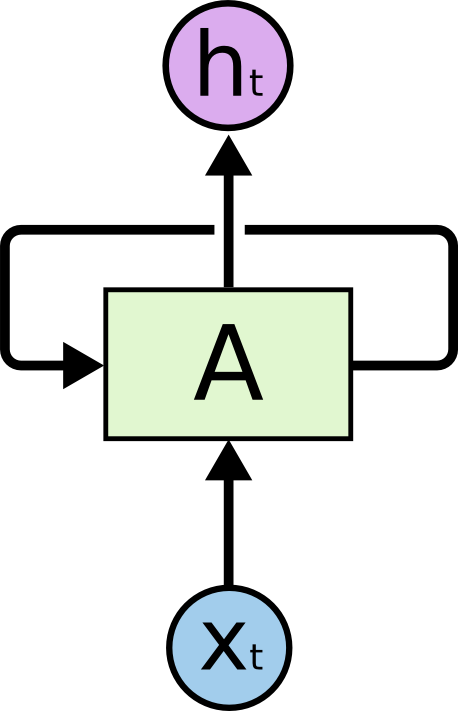
\includegraphics[width=.3\textwidth]{images/amir/RNN-rolled.png}%
     % you need to add the caption for the list of figures
    \caption[This is RNN cell image]{This is RNN cell}\label{fig:RNN cell}%
  \end{figure}
  \indent A recurrent neural network can be thought of as multiple copies of the same network, each passing a message to a successor. 

This chain-like nature reveals that recurrent neural networks. They’re the natural architecture of neural network to use for such data.\\
  \begin{figure}[H]%
    \center%
    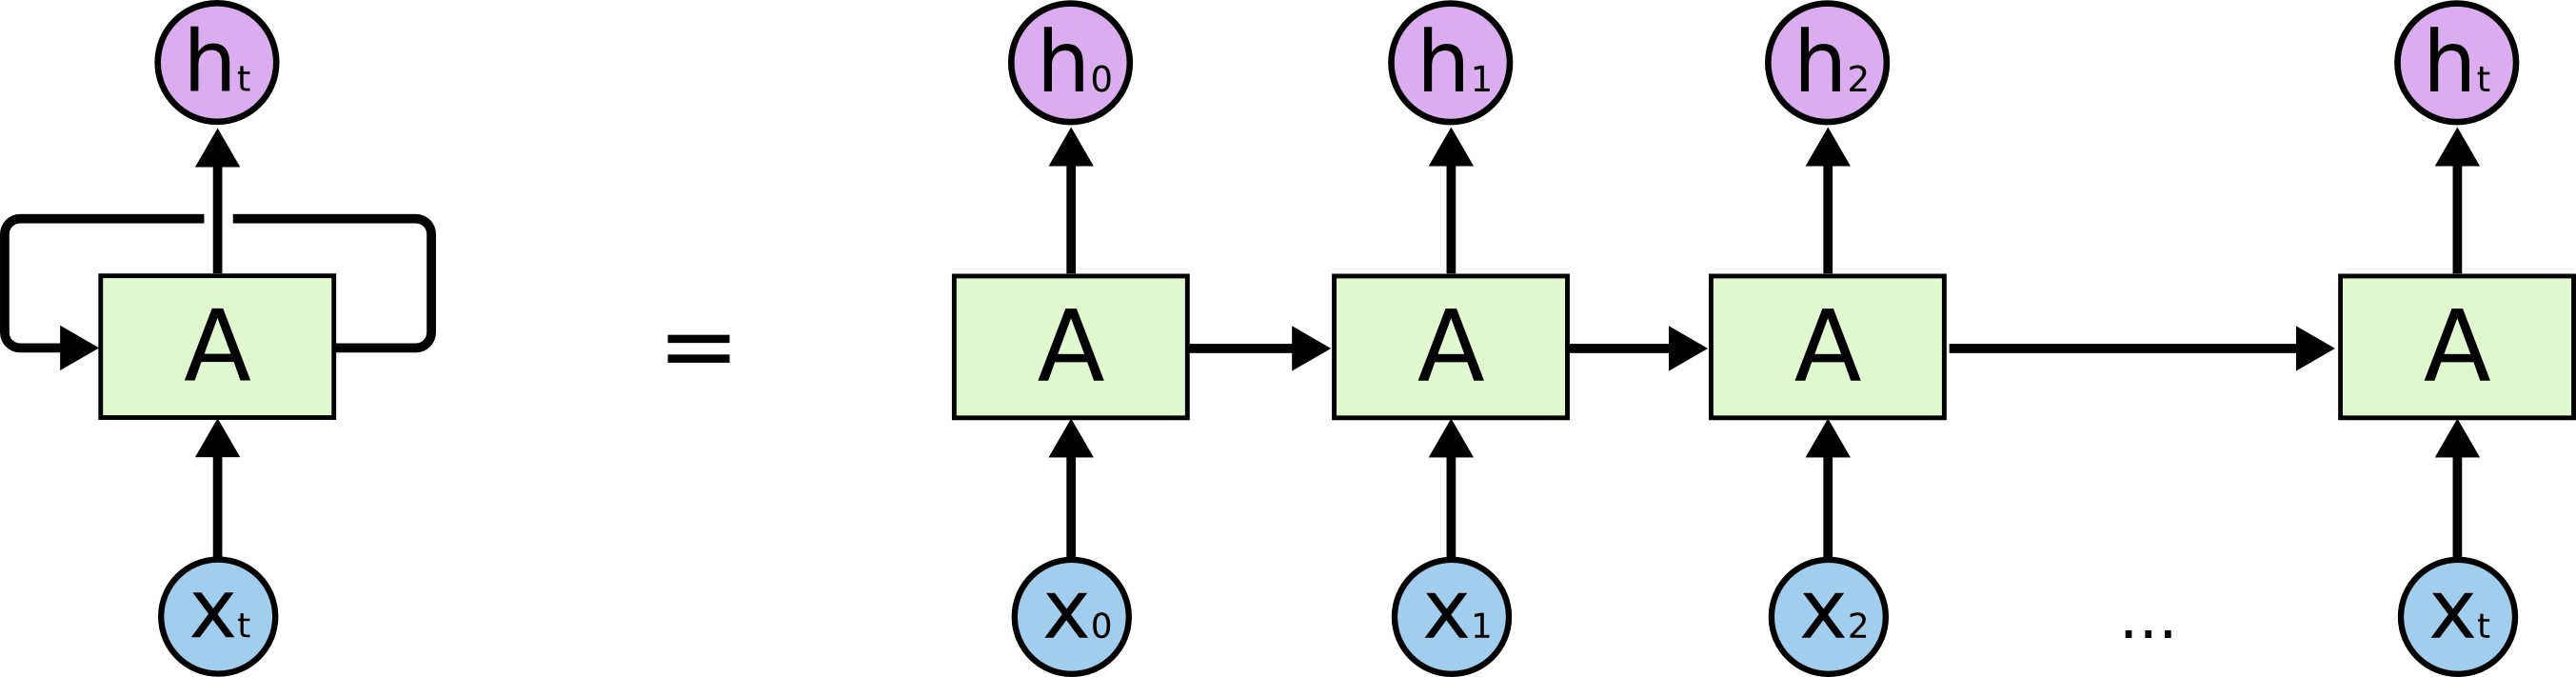
\includegraphics[width=\textwidth]{images/amir/RNN1-unrolled.png}%
     % you need to add the caption for the list of figures
    \caption[This is RNN net image]{chain-like recurrent neural network}\label{fig:RNN network}%
  \end{figure}
  
\subsection{The Problem of Long-Term Dependencies}
\indent One of the appeals of RNNs is the idea that they might be able to connect previous information to the present task, such as using previous video frames might inform the understanding of the present frame.\\
 \begin{figure}[H]%
    \center%
    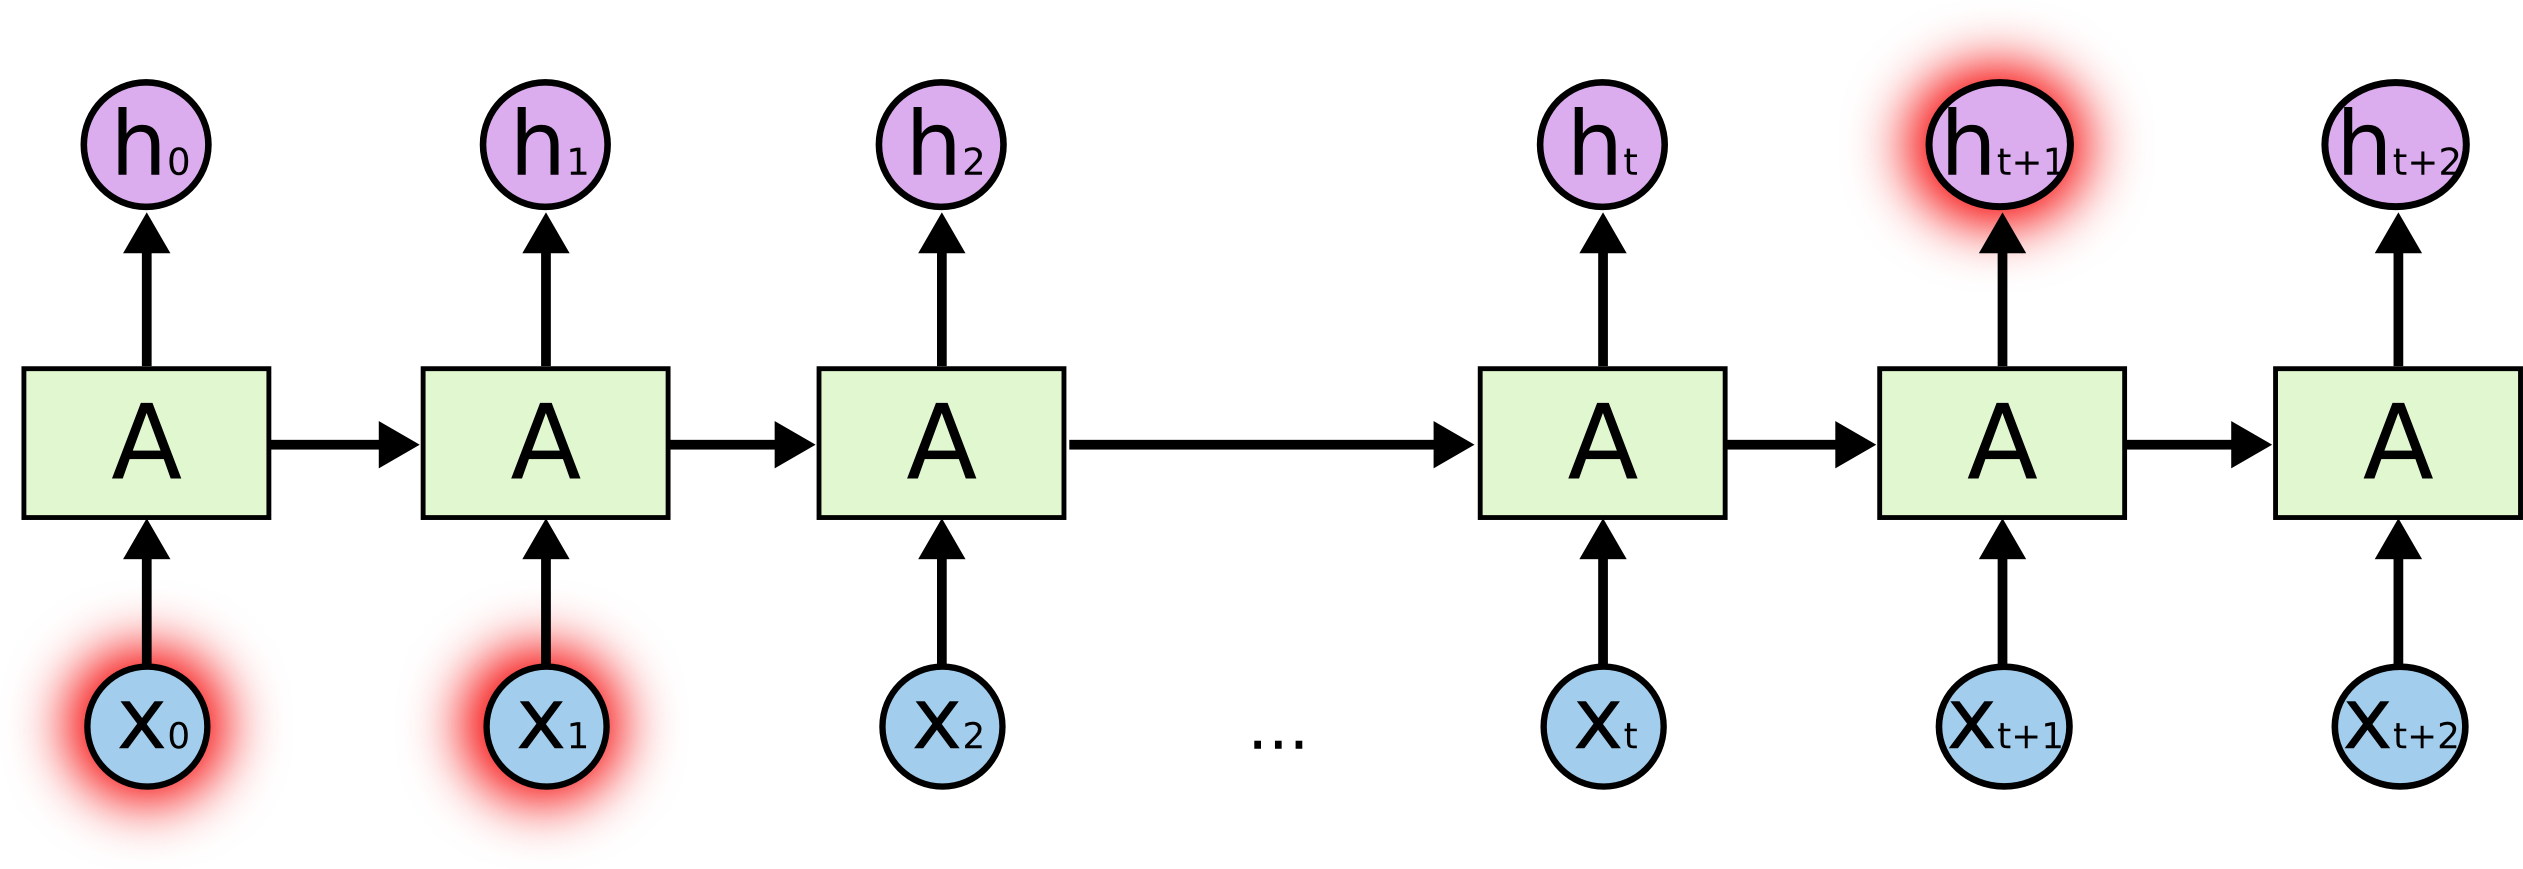
\includegraphics[width=\textwidth]{images/amir/RNN-longtermdependencies.png}%
     % you need to add the caption for the list of figures
    \caption[This is RNN net-dep image]{dependencies in recurrent neural network}\label{fig:RNN network-dep}%
  \end{figure}
  \indent If RNNs could do this, they’d be extremely useful. But can they? It depends.
Sometimes, we only need to look at recent information to perform the present task. For example, consider a language model trying to predict the next word based on the previous ones. If we are trying to predict the last word in “the clouds are in the sky,” we don’t need any further context – it’s pretty obvious the next word is going to be sky. In such cases, where the gap between the relevant information and the place that it’s needed is small, RNNs can learn to use the past information.But there are also cases where we need more context. Consider trying to predict the last word in the text “I grew up in France… I speak fluent French.” Recent information suggests that the next word is probably the name of a language, but if we want to narrow down which language, we need the context of France, from further back. It’s entirely possible for the gap between the relevant information and the point where it is needed to become very large.
\textit{Unfortunately, as that gap grows, RNNs become unable to learn to connect the information.}\\
\indent In theory, RNNs are absolutely capable of handling such “long-term dependencies.” A human could carefully pick parameters for them to solve toy problems of this form. Sadly, in practice, RNNs don’t seem to be able to learn them.The long term dependencies suffers from Vanishing Gradients or exploding ,those problems are solved by using LSTM or "Long-Short Term Memory" and GRU or "Gated Recurrent Unit"
\subsection{Types of RNN}
\begin{figure}[H]%
    \center%
    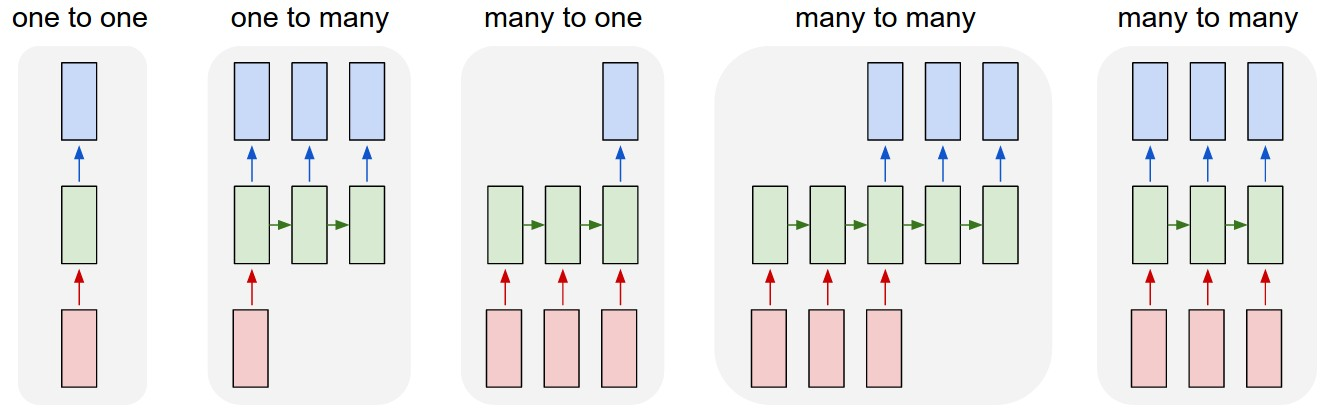
\includegraphics[width=\textwidth]{images/amir/diags.png}
     % you need to add the caption for the list of figures
    \caption[This is RNN types image]{different types of RNN nets}\label{fig:RNN types}%
  \end{figure}
\indent$\bullet$one2one:\\ is the ordinary network feedforward one.\\\\
\indent$\bullet$one2many:\\ is used in image captioning and recognition also in generating Music to generate one according to a number or something else.\\\\
\indent$\bullet$many2one:\\ is used in sentiment analysis to know if the sentence is positive or negative.\\\\
\indent$\bullet$many2many:\\ is used in machine translation.\\
\indent$\bullet$many2many:\\is used in language modelling also in video time-series analysis.\\\\
\subsection{Inside RNN Cell}
\begin{figure}[H]%
    \center%
    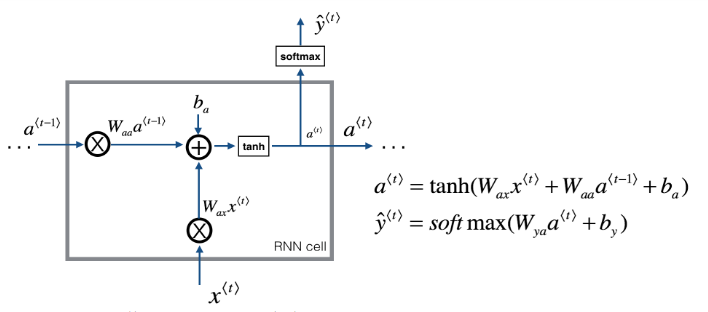
\includegraphics[width=.7\textwidth]{images/amir/Capture11.png}
     % you need to add the caption for the list of figures
    \caption[This is RNN inside image]{a look inside RNN cell}\label{fig:RNN inside}%
  \end{figure}
Basic RNN cell. Takes as input $x^t$ (current input) and $a^{(t-1)}$ (previous hidden state containing information from the past), and outputs $a^t$ which is 
given to the next RNN cell and also used to predict $y^t$hat.